\documentclass{sigchi}

% Use this section to set the ACM copyright statement (e.g. for
% preprints).  Consult the conference website for the camera-ready
% copyright statement.

% Copyright
\CopyrightYear{2016}
%\setcopyright{acmcopyright}
\setcopyright{acmlicensed}
%\setcopyright{rightsretained}
%\setcopyright{usgov}
%\setcopyright{usgovmixed}
%\setcopyright{cagov}
%\setcopyright{cagovmixed}
% DOI
\doi{http://dx.doi.org/10.475/123_4}
% ISBN
\isbn{123-4567-24-567/08/06}
%Conference
\conferenceinfo{CHI'16,}{May 07--12, 2016, San Jose, CA, USA}
%Price
\acmPrice{\$15.00}

% Use this command to override the default ACM copyright statement
% (e.g. for preprints).  Consult the conference website for the
% camera-ready copyright statement.

%% HOW TO OVERRIDE THE DEFAULT COPYRIGHT STRIP --
%% Please note you need to make sure the copy for your specific
%% license is used here!
% \toappear{
% Permission to make digital or hard copies of all or part of this work
% for personal or classroom use is granted without fee provided that
% copies are not made or distributed for profit or commercial advantage
% and that copies bear this notice and the full citation on the first
% page. Copyrights for components of this work owned by others than ACM
% must be honored. Abstracting with credit is permitted. To copy
% otherwise, or republish, to post on servers or to redistribute to
% lists, requires prior specific permission and/or a fee. Request
% permissions from \href{mailto:Permissions@acm.org}{Permissions@acm.org}. \\
% \emph{CHI '16},  May 07--12, 2016, San Jose, CA, USA \\
% ACM xxx-x-xxxx-xxxx-x/xx/xx\ldots \$15.00 \\
% DOI: \url{http://dx.doi.org/xx.xxxx/xxxxxxx.xxxxxxx}
% }

% Arabic page numbers for submission.  Remove this line to eliminate
% page numbers for the camera ready copy
% \pagenumbering{arabic}

% Load basic packages
\usepackage{balance}       % to better equalize the last page
\usepackage{graphics}      % for EPS, load graphicx instead 
\usepackage[T1]{fontenc}   % for umlauts and other diaeresis
\usepackage{txfonts}
\usepackage{mathptmx}
\usepackage[pdflang={en-US},pdftex]{hyperref}
\usepackage{color}
\usepackage{booktabs}
\usepackage{textcomp}

% Some optional stuff you might like/need.
\usepackage{microtype}        % Improved Tracking and Kerning
% \usepackage[all]{hypcap}    % Fixes bug in hyperref caption linking
\usepackage{ccicons}          % Cite your images correctly!
% \usepackage[utf8]{inputenc} % for a UTF8 editor only

% If you want to use todo notes, marginpars etc. during creation of
% your draft document, you have to enable the "chi_draft" option for
% the document class. To do this, change the very first line to:
% "\documentclass[chi_draft]{sigchi}". You can then place todo notes
% by using the "\todo{...}"  command. Make sure to disable the draft
% option again before submitting your final document.
\usepackage{todonotes}

% Paper metadata (use plain text, for PDF inclusion and later
% re-using, if desired).  Use \emtpyauthor when submitting for review
% so you remain anonymous.
\def\plaintitle{Git GUI Software Usability Survey}
\def\plainauthor{Victor Reginato, Erica Cheyne, Don Pham}
\def\emptyauthor{}
\def\plainkeywords{Authors' choice; of terms; separated; by
  semicolons; include commas, within terms only; required.}
\def\plaingeneralterms{Documentation, Standardization}

% llt: Define a global style for URLs, rather that the default one
\makeatletter
\def\url@leostyle{%
  \@ifundefined{selectfont}{
    \def\UrlFont{\sf}
  }{
    \def\UrlFont{\small\bf\ttfamily}
  }}
\makeatother
\urlstyle{leo}

% To make various LaTeX processors do the right thing with page size.
\def\pprw{8.5in}
\def\pprh{11in}
\special{papersize=\pprw,\pprh}
\setlength{\paperwidth}{\pprw}
\setlength{\paperheight}{\pprh}
\setlength{\pdfpagewidth}{\pprw}
\setlength{\pdfpageheight}{\pprh}

% Make sure hyperref comes last of your loaded packages, to give it a
% fighting chance of not being over-written, since its job is to
% redefine many LaTeX commands.
\definecolor{linkColor}{RGB}{6,125,233}
\hypersetup{%
  pdftitle={\plaintitle},
% Use \plainauthor for final version.
%  pdfauthor={\plainauthor},
  pdfauthor={\emptyauthor},
  pdfkeywords={\plainkeywords},
  pdfdisplaydoctitle=true, % For Accessibility
  bookmarksnumbered,
  pdfstartview={FitH},
  colorlinks,
  citecolor=black,
  filecolor=black,
  linkcolor=black,
  urlcolor=linkColor,
  breaklinks=true,
  hypertexnames=false
}

% create a shortcut to typeset table headings
% \newcommand\tabhead[1]{\small\textbf{#1}}

% End of preamble. Here it comes the document.
\begin{document}

\title{\plaintitle}

\numberofauthors{3}
\author{%
  \alignauthor{Victor Reginato\\
    \affaddr{McMaster University}\\
    \affaddr{Hamilton, Ontario}\\
    \email{reginavp@mcmaster.ca}}\\
  \alignauthor{Erica Cheyne\\
    \affaddr{McMaster University}\\
    \affaddr{Hamilton, Ontario}\\
    \email{cheyneem@mcmaster.ca}}\\
  \alignauthor{Don Pham\\
    \affaddr{McMaster University}\\
    \affaddr{Hamilton, Ontario}\\
    \email{phamd@mcmaster.ca}}\\
}

\maketitle

\begin{abstract}
  UPDATED---\today. This sample paper describes the formatting
  requirements for SIGCHI conference proceedings, and offers
  recommendations on writing for the worldwide SIGCHI
  readership. Please review this document even if you have submitted
  to SIGCHI conferences before, as some format details have changed
  relative to previous years. Abstracts should be about 150 words and
  are required.
\end{abstract}

\category{H.5.m.}{Information Interfaces and Presentation
  (e.g. HCI)}{Miscellaneous} \category{See
  \url{http://acm.org/about/class/1998/} for the full list of ACM
  classifiers. This section is required.}{}{}

\keywords{\plainkeywords}
  Git; gui.

\section{Introduction}
Git is a powerful version control system that is used by users of various
skill levels. This survey will evaluate 4 different Graphical User Interfaces (GUIs)
that help users manage their Git repositories.

 Each piece of software will be examined and reviewed based on a few different metrics including: what features it affords the 
user (what functions it provides)~\cite{Norman:2013}, how it signifies different affordances (how it shows
the user what they are able to do), the constraints present in the application
(things that the GUI prevents the user from doing), the feedback shown to the 
user when actions are performed and the overall discoverability of the GUI.
The conceptual model is also something that will be discussed for each GUI; how
it shows the underlaying conceptual model defined by Git will be evaluated.

The four Git GUIs that will be reviewed in this survey are by different companies and have
free versions available for public use. 

One client is GitHub, it is provided by Git Hub - a site that hosts git projects. It is a simplified GUI aimed at making git accessible to everyone
with a  reduced learning curve.

 GitKraken a client made by Axosoft, allows users to link to multiple remote repositories hosted on many types of servers (GitHub, BitBucket, etc...).
It provides access to many of Git's functions, making it useful for advanced users.

The third piece of software to be reviewed is SmartGit. SmartGit allows for almost ALL of gits
features to be used, making it useful in almost any git scenario. 

Source tree is the last piece of software that will be examined in this survey. SourceTree was developed by Atlassian and
prides itself on it's ability to communicate information about the state of a repository to the user.

\section{Git User Goals and Git Terms Explained}
Each of the reviews in this document will contain a brief introduction to the software and some notable features, before applying 
the terms previously introduced to two main high-level tasks. Those tasks will be clearly identified 
after stating why someone might want to use Git and providing an idea of the benefits that Git gives to the user.

Users of Git in general want to be able to make changes to their code and have a centralized version of the code reflect those changes. 
The ability to view when a change (in the form of what's called a 'commit') to the code, when that
commit happened, and who made those changes can prove to be an invaluable debugging tool
should the software malfunction after a commit is made. When work needs to be done on a 
separate feature of an application, branching (the process of copying the code to be modified
independently of other branches) is critical for testing and developing features alongside an application.

There are two core tasks that almost all Git users will perform. The first task is making changes to a local copy of the code,
committing those changes, and finally pushing those changes to the master branch. This task should 
provide appropriate feedback to the user in the case that they are unable to push for whatever reason.
The second task is a common and can be a more involved task, merging a branch into the master branch. 
When the user creates a branch from the master to add a feature, or fix a bug (programming error), they
will eventually need to merge that branch back into the master for it to be integrated into the main application. 
This process can involve many merge conflicts (when the differences in source code between two revisions of
a file cannot be automatically resolved) that can make this challenging.

 These high level goals can be broken down into Git commands, the GUIs use Git commands to achieve the user's goals. Depending on the GUI,
it is explicit about the git commands that will be used and will allow the user to customize them. 

\section{GitHub Desktop Review}
This section reviews GitHub desktop, the default GUI for managing git repositories.
This application is produced by GitHub and can be downloaded and opened directly from 
their website. The affordance that most git users appreciate about GitHub desktop over 
other applications is the easy cloning ability. This interface does not allow for users 
to edit their code directly within the app, nor can you view the most recent version of 
the files. Instead you can see the initial files, and you can see the specific changes
that you made to the files. In order to see the current file with all changes applied
and to make changes to the file you must open those files in another program on your 
machine. This application does allow the user to see all changes that were made to a file, 
as well as who made those changes.
 
\subsection{Stage, Commit and Push Changes to Remote}
Being able to take changes made on the users machine and apply them to the remote repository 
is an essential element to managing a git repository. This is described for GitHub desktop in
the HTA ***called this***. After a user has made a change to a file on their machine and has 
opened the GitHub desktop application, they must choose what repository they have made changes 
to. The repositories are found on the left hand side of the page and although there is no title 
signifying that these are the repositories, the filter repositories field is used as a signifier.
The feedback the user receives after pressing the repository name is not immediate and could be
frustrating depending on how long the repository takes to load. 

The user must then enter the changes view, signified by the dot appearing on the changes 
button. In this view all changes on the local machine are automatically selected, but none of the 
changes are automatically visible. This can lead to a misconception when users enter their summary
of the change, believing they are writing the description for one change but actually committing 
all changes with that summary. This is a problem with discoverability in the system, a user might 
make this mistake many times before realizing their actions consequences. After a user commits their 
changes, they receive a small piece of feedback at the bottom. Unfortunately this is the same colour 
as the rest of the GUI and is not very noticeable.

There is another problem in discoverability for this process. This comes from the actual push action 
and closes off the action described in the HTA. Namely, GitHub users the word push to describe 
pushing a change from your local repository onto the remote repository. However, in GitHub desktop,
this action is instigated by pressing the sync button in the right hand corner. A long term git user
could have trouble relearning the new terminology or locating the button in the first place. 

\subsection{Merge a Branch into Master}
Another important function to enable a user to manage their repository is being able to merge two 
branches, specifically merging a branch into the master branch. This is described in the HTA 
***name of HTA***. The whole process in GitHub Desktop has problems with discoverability. In order 
to merge a branch into master you must have selected the master branch, and then select the branch 
you wish to merge into master. This is counter intuitive as the user is most likely in their branch 
already and would have to switch to master in order to achieve this goal. The last action that the user
must take is to press the update button. This lessens the discoverability of the GUI because once again
this is not the terminology that GitHub traditionally uses.

\section{Git Kraken Review}
GitKraken is a powerful Git GUI that was meant aimed at making basic Git tasks easier for developers.
One of the first things to note about GitKraken is the walk through it gives you upon the
first startup of the application. It highlights some of the basic ways that GitKraken integrates with Git by
using signifiers (text boxes) to point to different buttons and explain what each button affords the user.
It also outlines some basic startup tasks including: how to link to your existing GitHub profile, how to change
account preferences, and how to add an existing repository.

Upon opening a repository to explore, you are shown a commit history graph. The graph affords the viewing of 
the impact of each commit on the central code base. It shows when it was committed, who pushed it and
the modifications made in that commit. The visual representation that it provides aids in showing the 
conceptual model that Git gives to repositories; branches are shown as physical branches and visually indicate
at what commit they branched off of the code.

\begin{figure*}
  \centering
  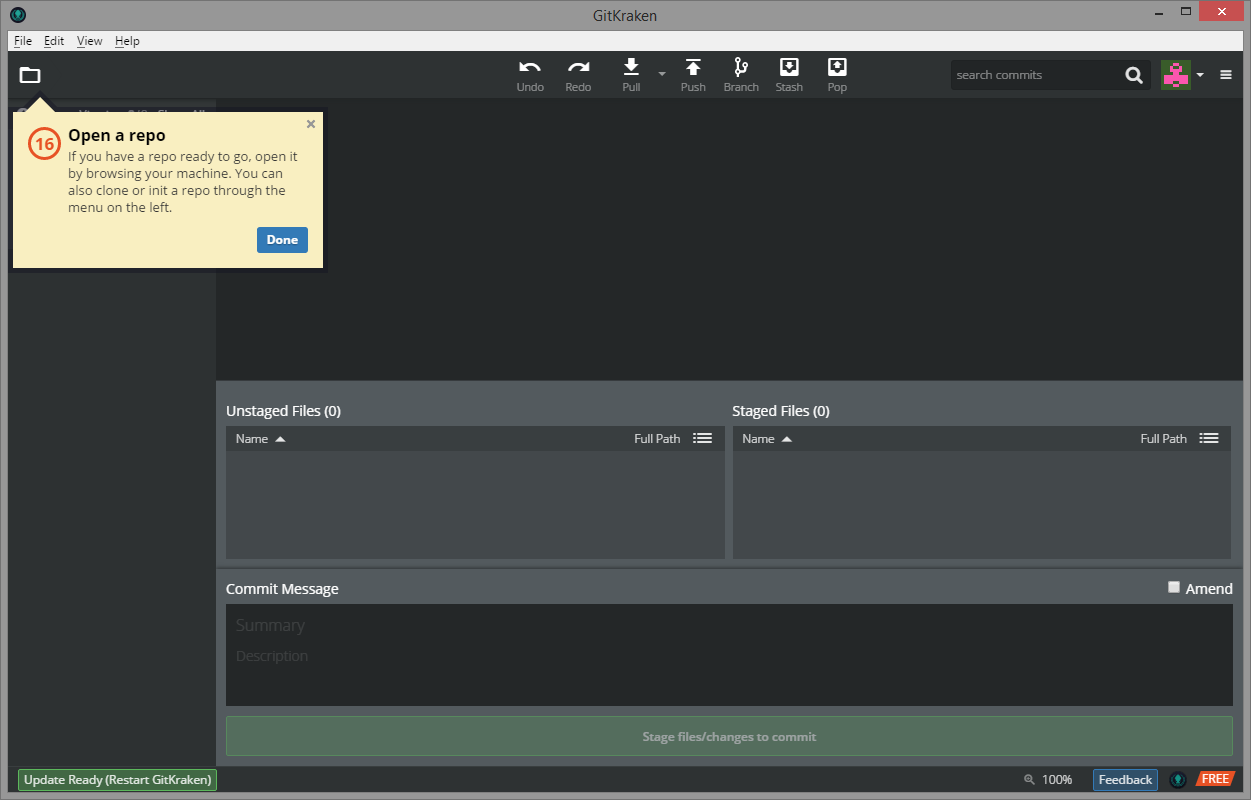
\includegraphics[width=1.75\columnwidth]{figures/GitKraken/Open_a_repo}
  \caption{This image is a screen shot of the GitKraken tutorial that happens on the first startup, it shows how to open/change repos}~\label{fig:GitKrakenFigure1}
\end{figure*}

\subsection{Stage, Commit and Push Changes to Remote}
This subsection will go over the task outlined in the GitKrakenHTA1 - the task of staging committing 
and pushing changes to a remote. Images will be provided to supplement the critique. 

The first item, 1.1., is very simple in GitKraken, as it affords the switching of local repositories by clicking the folder
 in the top left corner. It signifies that you can click the folder by changing the cursor, which is not a very clear signifier 
as you need to hover your mouse over it to see that you can click it. Without the tutorial, this would have been difficult to discover.

1.2 is also quite simple, selecting the desired branch within a repository can be done by hovering over it under the 
'local' heading with your mouse, clicking the three vertical dots that appear (or by more intuitively, right clicking anywhere over the branch name) 
and selecting checkout from the drop down.

1.3 in the HTA is somewhat intuitive. To view the changes you have made locally, you can select the top item in
the branch which is highlighted. GitKraken indicates that there are uncommitted changes by having a dashed circle as apposed to a solid circle.
After you have done that, you can see all the files with changes made on the right side of the screen.
GitKraken affords the viewing of changes by clicking on the files, the changes are shown in the middle of the screen and the additions and subtractions are signified by being highlighted green or red (this uses a cultural convention relating to traffic lights ~\cite{Norman:2013}). 

1.4 To stage all changes in a file you can click on the green plus next to the file name in the unstaged files preview window. When reviewing the changes in the file you have the option of staging or unstaging hunks. A hunk is a logical grouping of changes based on proximity within a file. GitKraken affords limited editing before staging a file by allowing you to add or remove hunks. It does not however allow you to edit the file otherwise, line by line changes cannot be discarded or added.
The green button at the bottom right shows you what you need to do next to push. When you are reviewing changes, and staging files, it displays the text "Stage files/changes to commit". It does not afford clicking and signifies that you cannot click it by graying out the button and changing your mouse cursor. This decreases the discoverability by providing little to no obvious feedback to the use; instead of graying out the button, it should not allow the user to perform the operation when clicked and let them know what still needs to be done by showing an error message. This constraint makes sense only in the context of what Git can and cannot do (it can't commit without a commit message or any staged changes), not in the sense of what the user wants to do.

1.5 pushing changes to the remote branch is simple after writing a commit message and staging all changes, however it does not afford using some of Git's more powerful pushing options. For example, if you wanted to forcibly change the HEAD (The commit that it points to) of the remote branch, there is no option to do so. When you try to push and the local repo is out of date, you must pull. Upon pulling an encountering a merge conflict, you are allowed to make line by line changes, which is not especially intuitive considering you were not able to do so at the staging level.

\begin{figure*}
  \centering
  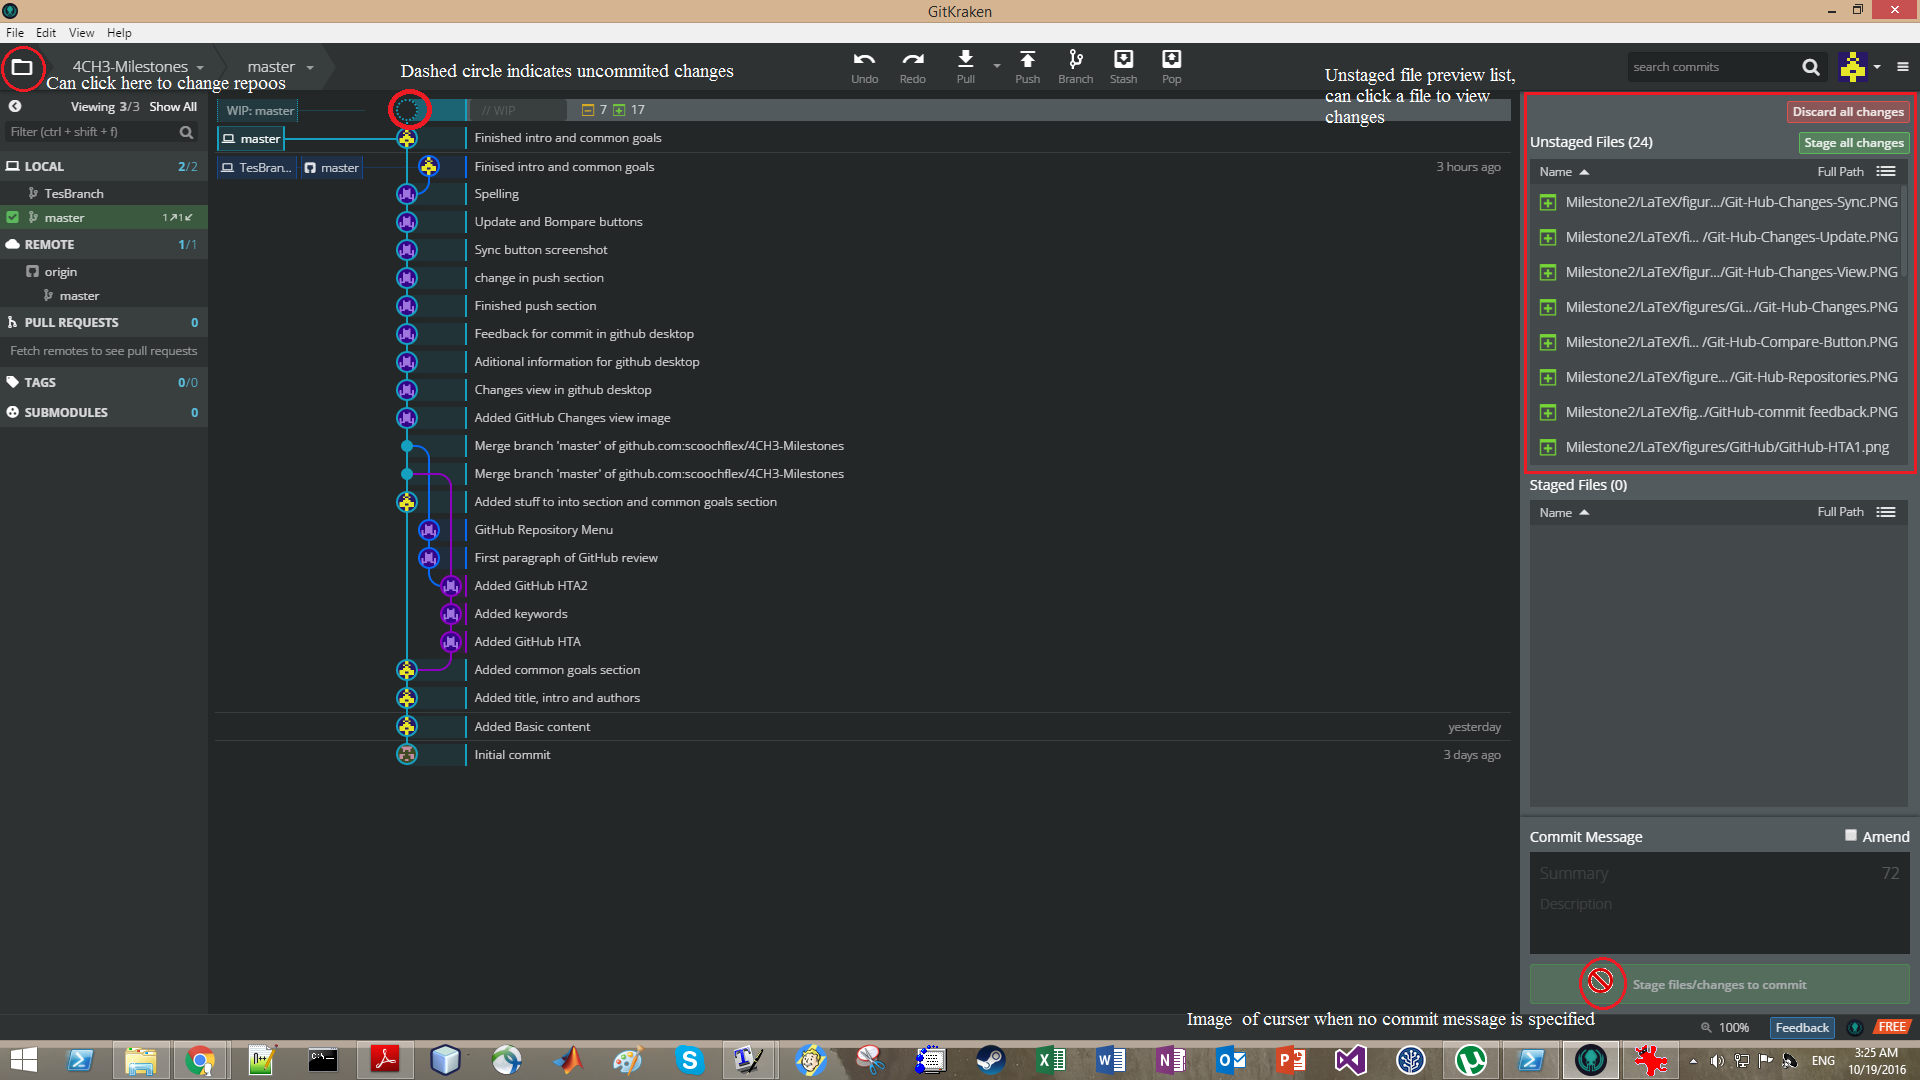
\includegraphics[width=1.75\columnwidth]{figures/GitKraken/ScreenshotHighlighted}
  \caption{This image is a screen shot of the GitKraken window with some features highlighted}~\label{fig:GitKrakenFigure2}
\end{figure*}

\begin{figure*}
  \centering
  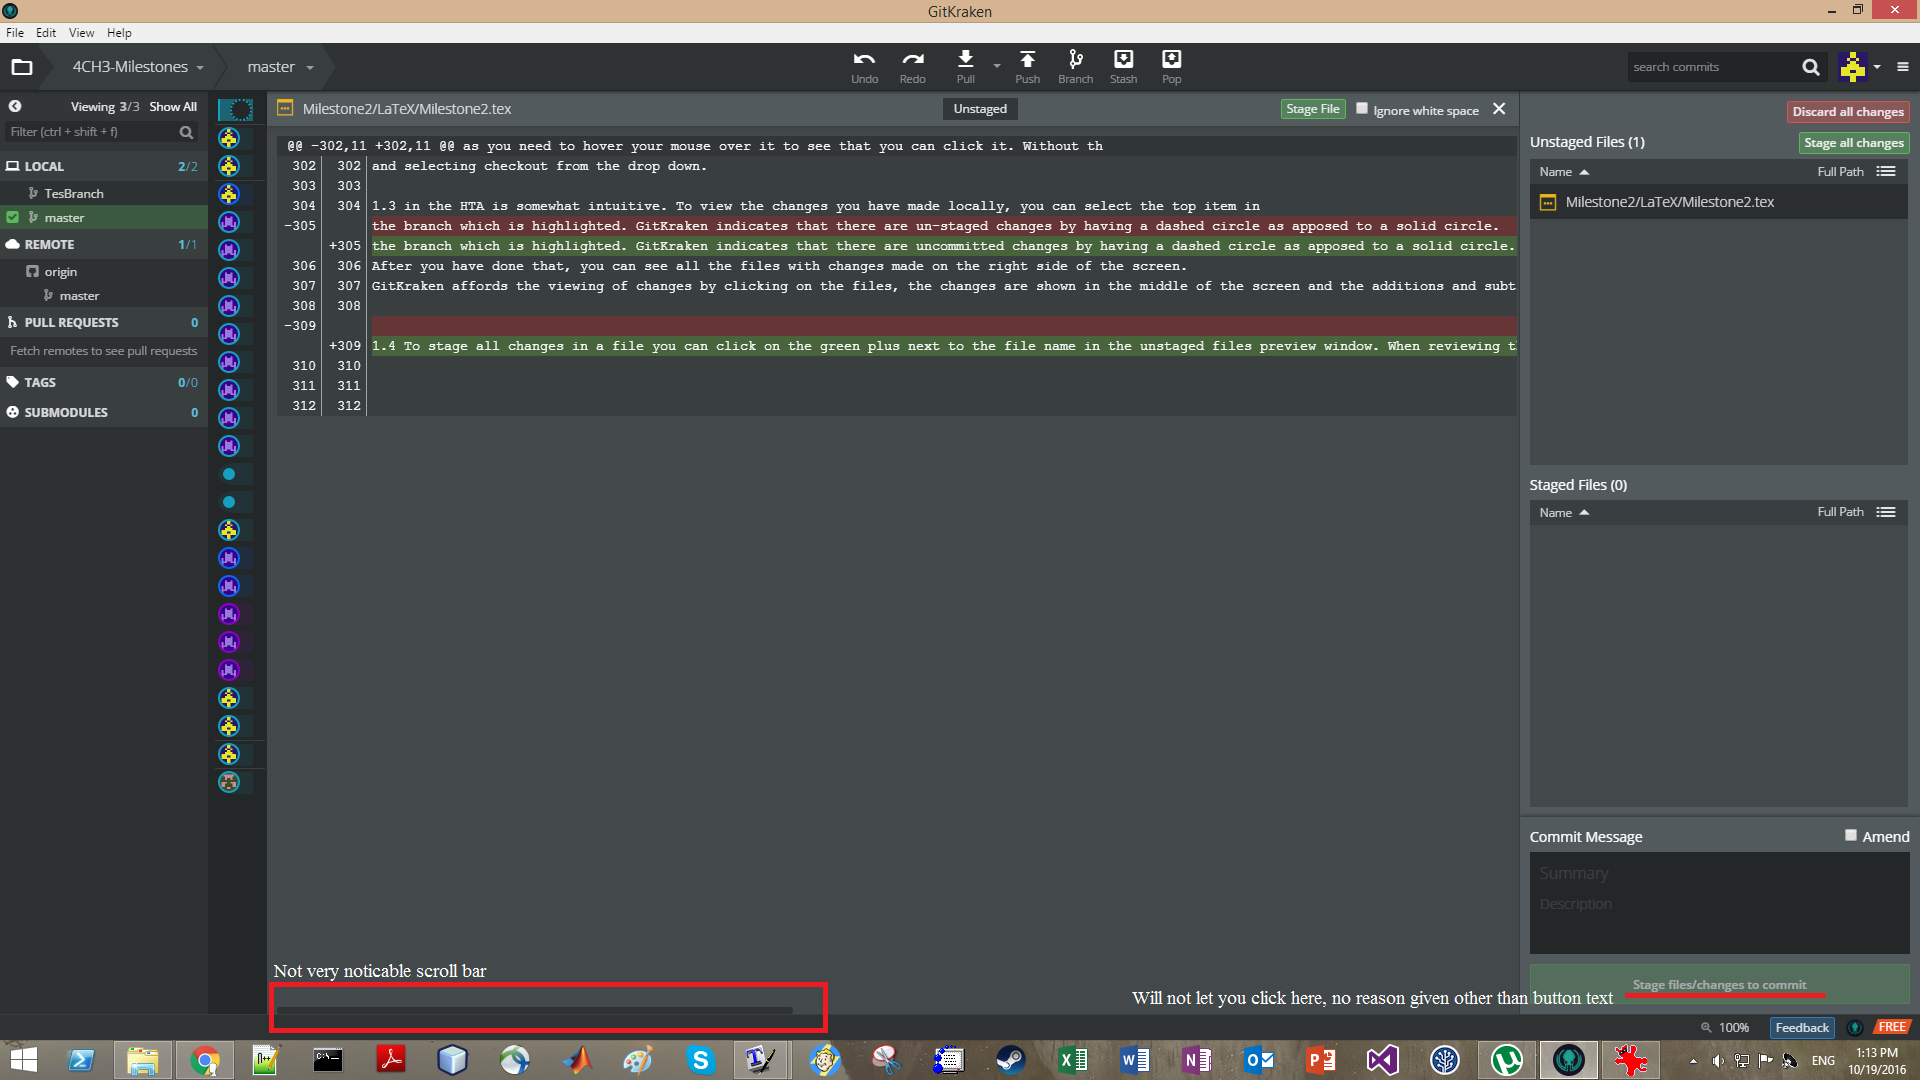
\includegraphics[width=1.75\columnwidth]{figures/GitKraken/Screenshot2Highlighted}
  \caption{This image is a screen shot of the GitKraken with some issues discussed that have been highlighted}~\label{fig:GitKrakenFigure3}
\end{figure*}

\subsection{Merge a Branch into Master}
When you are working off of two different branches, you will eventually need to merge the two together.
This is a core task in the Git development process. This section will briefly elaborate on the GitKrakenHTA2 steps and critique elements that could have been done better.

2.1 The details of checking out a branch have already been covered.

2.2 The details of selecting a branch to merge has also already been covered.

2.3. The resolution of merge conflicts in GitKraken is somewhat streamlined. It allows you to line by line go through the changes and shows a preview of the result of the merge for each file in conflict. This also be quite tedious if you are working with large files. GitKraken does not allow you to specify the way it will attempt to automatically resolve conflicts (theirs, ours, etc...). In this sense, it is not quite as powerful as it first seems. This constraint on what it allows users to do is unnecessary, as they can explain different merge strategies to new users with little effort and have a default strategy set.

2.4 Writing a commit message when resolving a merge is not different from writing a message when committing staged changes.

2.5 You also have the option of aborting the merge which can be nice, but is also a bit dangerous as it allows the user to completely disregard all resolutions they may have already manually made.

\begin{figure*}
  \centering
  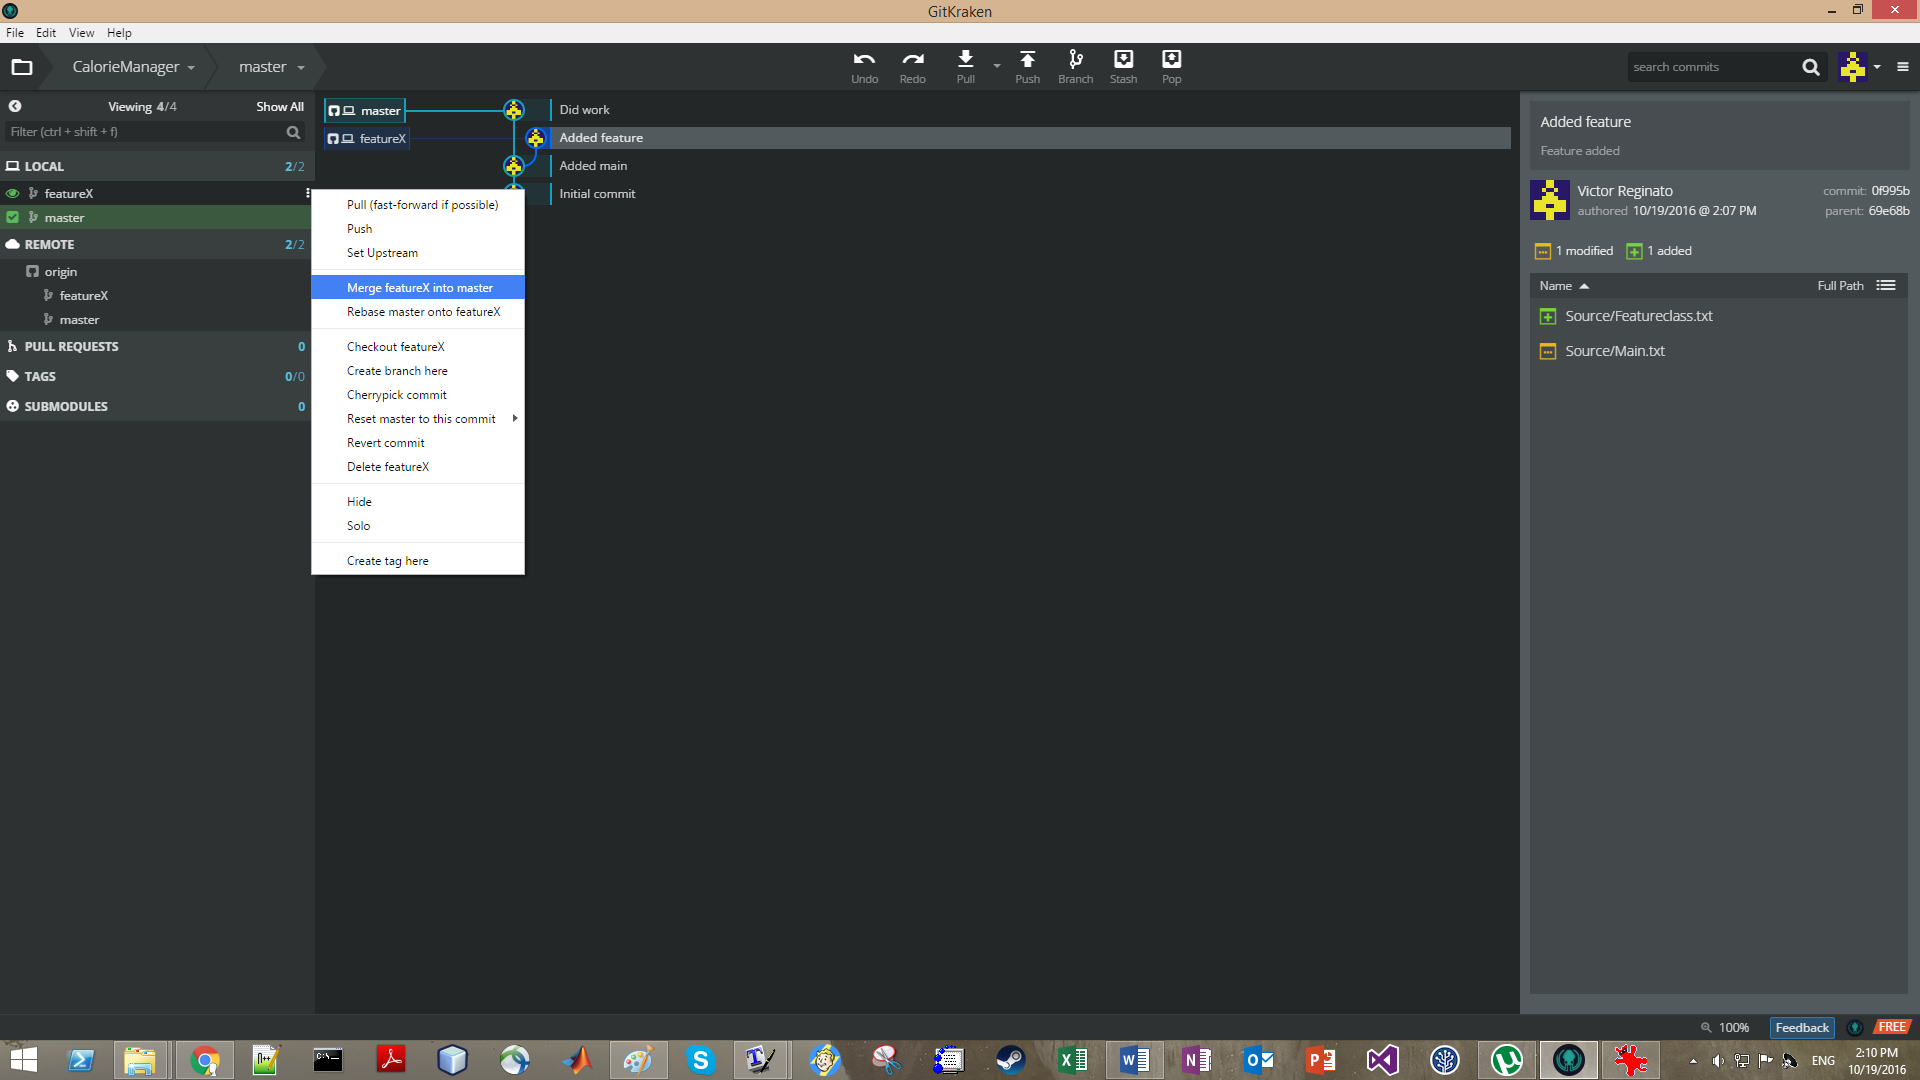
\includegraphics[width=1.75\columnwidth]{figures/GitKraken/MergeDropdown}
  \caption{This image is a screen shot of the GitKraken showing how to access a merge between two branches}~\label{fig:GitKrakenFigure4}
\end{figure*}

\begin{figure*}
  \centering
  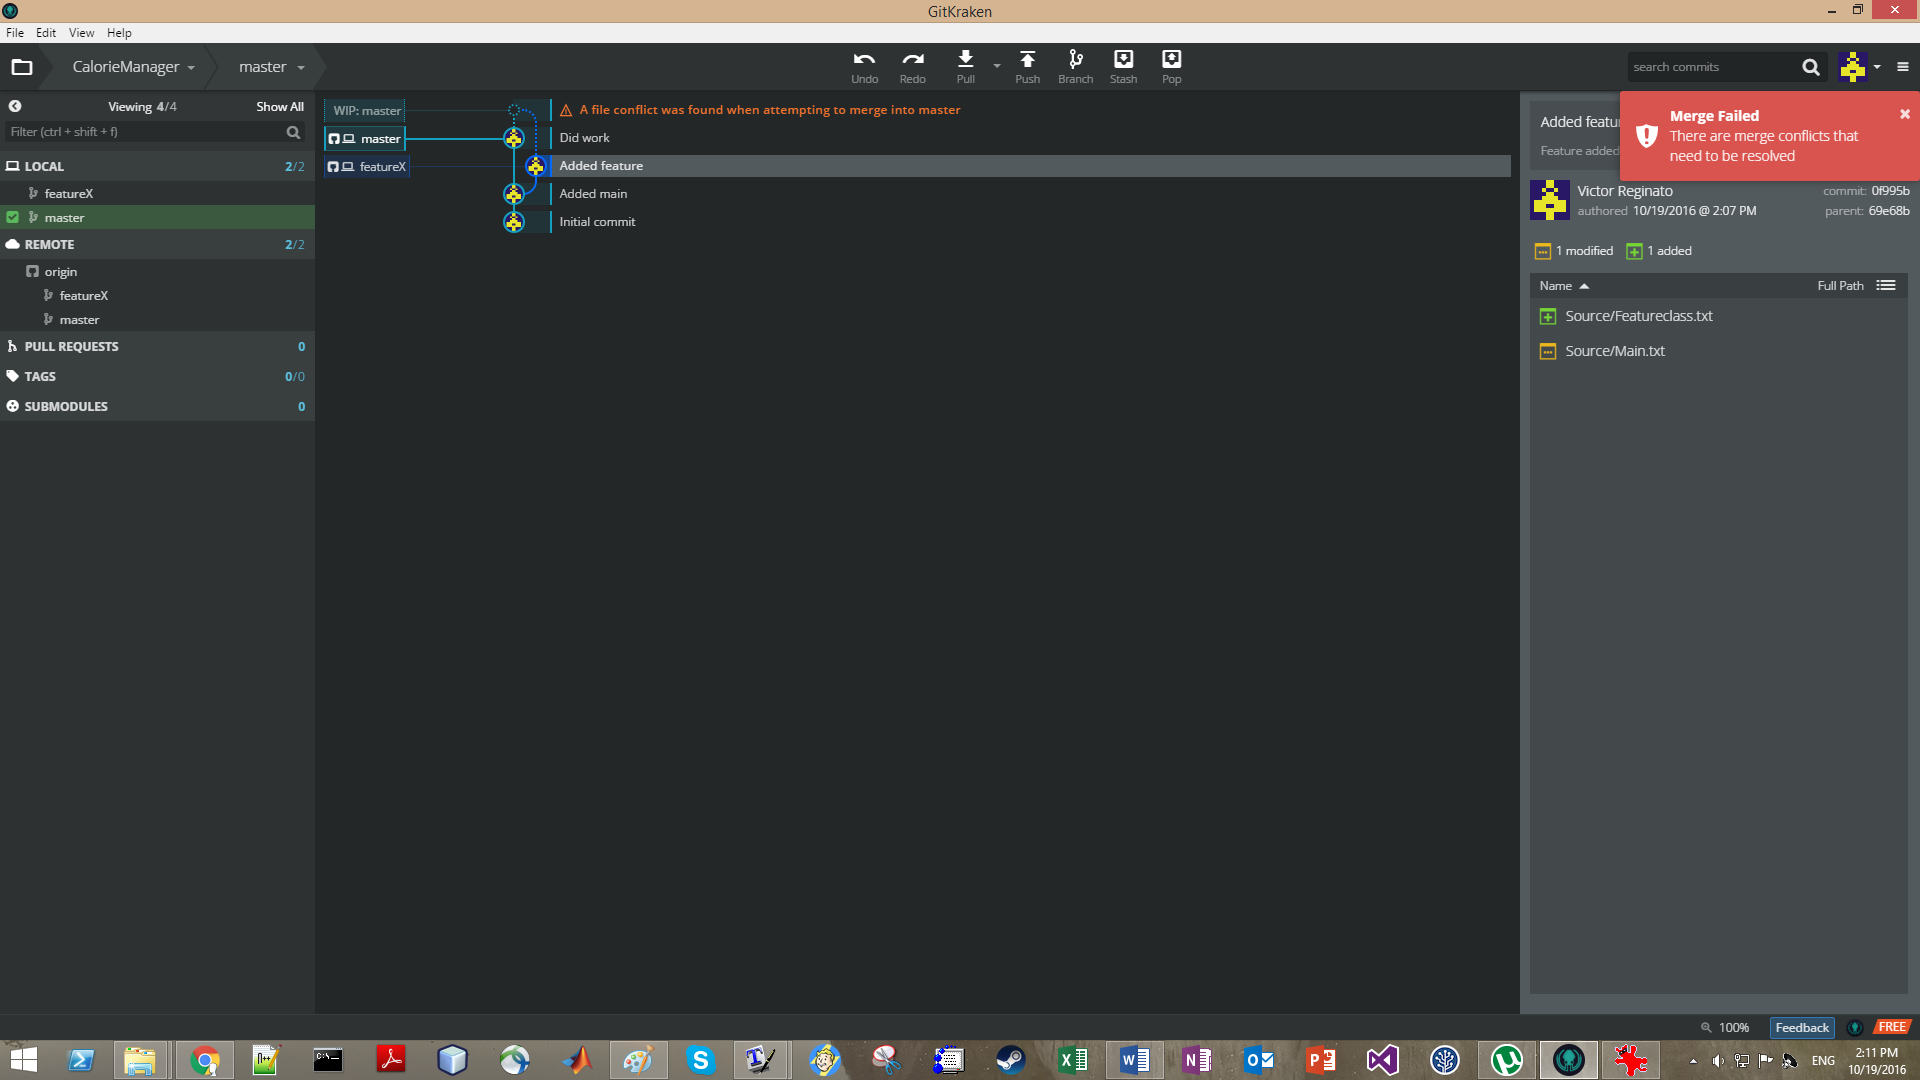
\includegraphics[width=1.75\columnwidth]{figures/GitKraken/MergeFailedNotification}
  \caption{This image is a screen shot of the GitKraken showing what a failed merge looks like}~\label{fig:GitKrakenFigure5}
\end{figure*}

\begin{figure*}
  \centering
  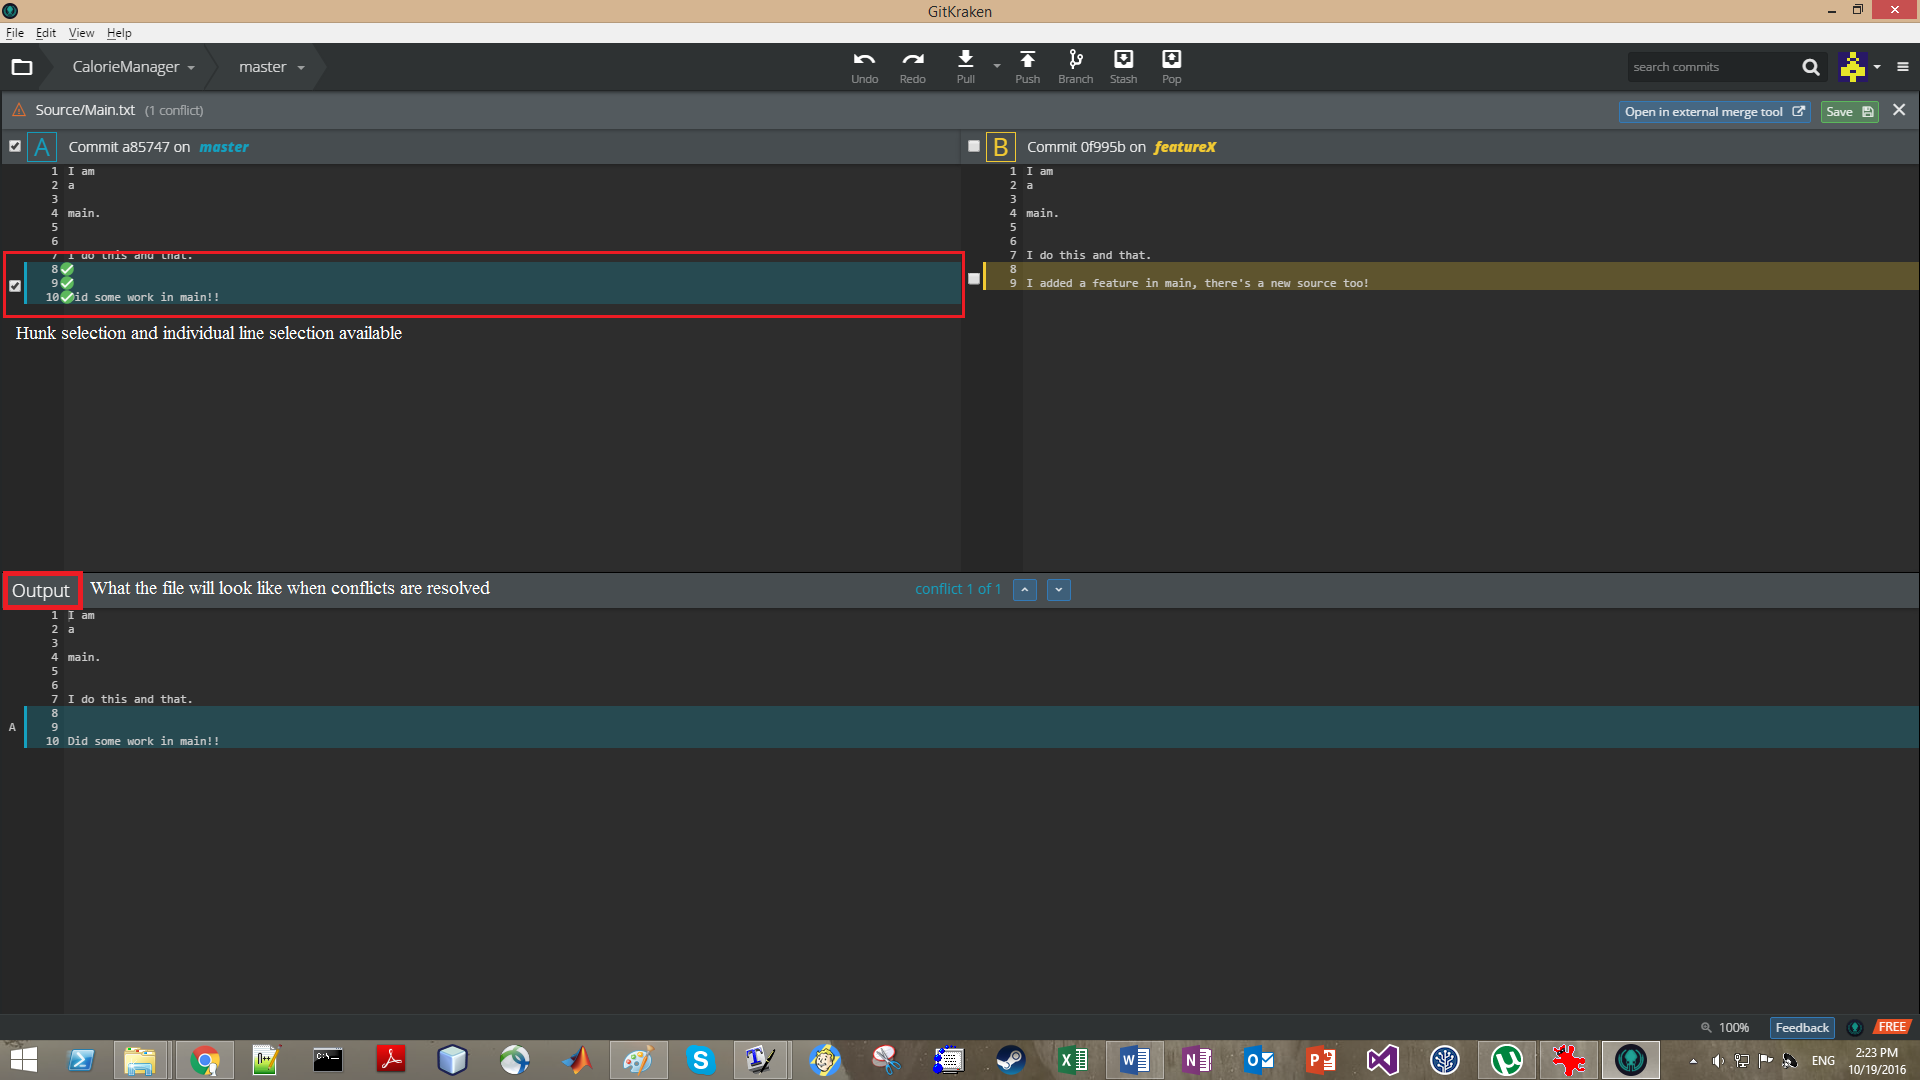
\includegraphics[width=1.75\columnwidth]{figures/GitKraken/MergeConflictResolution}
  \caption{This image is a screen shot of the GitKraken showing how to resolve conflicts}~\label{fig:GitKrakenFigure6}
\end{figure*}

\section{SmartGit}
SmartGit is another



\section{Conclusion}
It is important that you write for the SIGCHI audience. Please read
previous years' proceedings to understand the writing style and
conventions that successful authors have used. It is particularly
important that you state clearly what you have done, not merely what
you plan to do, and explain how your work is different from previously
published work, i.e., the unique contribution that your work makes to
the field. Please consider what the reader will learn from your
submission, and how they will find your work useful. If you write with
these questions in mind, your work is more likely to be successful,
both in being accepted into the conference, and in influencing the
work of our field.

\begin{figure*}
  \centering
  \includegraphics[width=1.75\columnwidth]{figures/GitKraken/GitKrakenHTA1}
  \caption{This image is a screen shot of the GitKraken happens on the first startup}~\label{fig:GitKrakenHTA1}
\end{figure*}

\begin{figure*}
  \centering
  \includegraphics[width=1.75\columnwidth]{figures/GitKraken/GitKrakenHTA2}
  \caption{This image is a screen shot of the GitKraken window with some features highlighted}~\label{fig:GitKrakenHTA2}
\end{figure*}


% BALANCE COLUMNS
\balance{}

% REFERENCES FORMAT
% References must be the same font size as other body text.
\bibliographystyle{SIGCHI-Reference-Format}
\bibliography{sample}

\end{document}

%%% Local Variables:
%%% mode: latex
%%% TeX-master: t
%%% End:
